\paragraph{(a)}
Sea $f\colon\bC^{2m}\to\bC$ dada por $f(x,y)=x^*y$ (nota: el enunciado dice $x^ty$, que no es exactamente el producto interno en $\bC$, pero la demostración es la misma). El algoritmo $\tilde{f}:\mathbb{F}^{2m}\to\mathbb{F}$ de producto interno está dado por
\[
	\tilde{f}(x,y)=fl\left(\sum_{k=1}^m fl(\bar{x}_ky_k)\right)
\]

Dados $x,y\in\bC^m$, existen $\epsilon_1,\dotsc,\epsilon_m$ con $|\epsilon_k|\leq\epsilon_{m\'aq}$, donde $\epsilon_{m\'aq}$ es el épsilon de la máquina, tales que $fl(\bar{x}_ky_k)=\bar{x}_ky_k(1+\epsilon_k)$. Además, existe $\epsilon_{m+1}$ con $|\epsilon_{m+1}|\leq\epsilon_{m\'aq}$ tal que
\[
	fl\left(\sum_{k=1}^m fl(\bar{x}_ky_k)\right)=\left(\sum_{k=1}^m fl(\bar{x}_ky_k)\right)(1+\epsilon_{m+1})
\]
Combinando lo anterior, obetenemos que
\[
	\tilde{f}(x,y)=\sum_{k=1}^m \bar{x}_ky_k(1+\epsilon_{k})(1+\epsilon_{m+1})
\]
y el error es
\begin{align*}
	|\tilde{f}(x,y)-f(x,y)|&=\left|\sum_{k=1}^m \bar{x}_ky_k(\epsilon_{k}+\epsilon_{m+1}+\epsilon_k\epsilon_{m+1})\right|\\
	&\leq\Vert x\Vert_2\left(\sum_{k=1}^m|y_k|^2\,|\epsilon_k+\epsilon_{m+1}+\epsilon_k\epsilon_{m+1}|^2\right)^{\frac{1}{2}}&\text{(desig. Cauchy-Schwartz)}\\
	&\leq\Vert x\Vert_2\left(\sum_{k=1}^m|y_k|^2\,(|\epsilon_k|+|\epsilon_{m+1}|+|\epsilon_k\epsilon_{m+1}|)^2\right)^{\frac{1}{2}}\\
	&\leq\Vert x\Vert_2\left(\sum_{k=1}^m|y_k|^2\,(2|\epsilon_{m\'aq}|+|\epsilon_{m\'aq}|^2)^2\right)^{\frac{1}{2}}\\
	&=\Vert x\Vert_2\Vert y\Vert_2(2|\epsilon_{m\'aq}|+|\epsilon_{m\'aq}|^2)
\end{align*}
de manera que
\[
	\frac{|\tilde{f}(x,y)-f(x,y)|}{\Vert x\Vert_2\Vert y\Vert_2}\leq 2|\epsilon_{m\'aq}|+|\epsilon_{m\'aq}|^2=O(\epsilon_{m\'aq})
\]

Dados $x,y\in\bC^{m}\setminus\{0\}$, existe $i$ tal que $\sqrt{m}|x_i|\geq\Vert x\Vert_2$ (precisamente, $i$ tal que $|x_i|=\Vert x\Vert_\infty$). Defina $\tilde{x},\tilde{y}$ dados por
\begin{align*}
	\tilde{x}_k&=x_k\qquad\forall k=1,\dotsc,m\\[1ex]
	\tilde{y}_k&=y_k\qquad k\neq i\\[1ex]
	\tilde{y}_i&=
		\frac{1}{\bar{x}_i}\Bigl(\tilde{f}(x,y)-\sum_{l\neq i}\bar{x}_ly_l\Bigr)
\end{align*}
note que evidentemente $f(\tilde{x},\tilde{y})=\tilde{f}(x,y)$. Vea que el error entre $\tilde{y}$ y $y$ es igual a
\[
	\frac{\Vert \tilde{y}-y\Vert_2}{\Vert y\Vert_2} =\frac{|\tilde{y}_i-y_i|}{\Vert y\Vert_2} =\frac{|\tilde{f}(x,y)-f(x,y)|}{|x_i|\Vert y\Vert_2}
	\leq\sqrt{m}\frac{|\tilde{f}(x,y)-f(x,y)|}{\Vert x\Vert_2\Vert y\Vert_2} =O(\epsilon_{m\'aq})
\]

Claramente $\dfrac{\Vert\tilde{x}-x\Vert_2}{\Vert x\Vert_2}=0=O(\epsilon_{m\'aq})$.

\smallskip
$\therefore$ El algoritmo $\tilde{f}$ es estable para atrás.
\paragraph{(b) Efectos del factor de crecimiento:}
\subparagraph{(a)} \strut

\lstinputlisting{../codigo/matrizPatologica.m}

\subparagraph{(b)} Al correr el siguiente código
\lstinputlisting[numbers=none]{../codigo/ejer6bb.m}
se obtuvo que el factor de crecimiento es aproximadamente $5.629\times10^{14}$ y la norma es $0$.

Es fácil notar que la descomposición $LU$ de $A$ está dada por
\[
	L=\begin{bmatrix}
		1      & 0      & 0      & \cdots & 0      \\
		-1     & 1      & 0      & \cdots & 0      \\
		-1     & -1     & 1      & \cdots & 0      \\
		\vdots & \vdots & \vdots & \ddots & \vdots \\
		-1     & -1     & -1     & \cdots & 1
	\end{bmatrix}
	\quad\text{y}\quad
	U = \begin{bmatrix}
		1      & 0      & 0      & \cdots & 0      & 1      \\
		0      & 1      & 0      & \cdots & 0      & 2      \\
		0      & 0      & 1      & \cdots & 0      & 4      \\
		\vdots & \vdots & \vdots & \ddots & \vdots & \vdots \\
		0      & 0      & 0      & \cdots & 1      & 2^{48} \\
		0      & 0      & 0      & \cdots & 0      & 2^{49}
	\end{bmatrix}
\]
y vemos que $\rho(A)=2^{49}\approx5.629\times10^{14}$, que es el resultado que habíamos obtenido antes.

Recuerde que la aritmética de precisión doble puede representar de manera exacta potencias de 2 hasta $2^{1023}$, por lo que la matriz $U$ es almacenable de forma exacta. Al calcular el producto $LU$ el peor caso posible sucede al calcular la esquina inferior derecha, se debe realizar la sumatoria
\[
	-1-2-4-8-\dotsb-2^{48}+2^{49}
\]
que la computadora calcula asociando a la izquierda, y puesto que en ningún paso de esta sumatoria, el número es una potencia de 2, es posible que haya errores de redondeo. Sin embargo, recuerde también que la precisión doble posee 53 dígitos significativos (52 dígitos de mantisa más un dígito de parte entera), mientras que el número $-1-2-4-\dotsb-2^{48}$ tiene 49 dígitos significativos, por lo que es posible almacenarlo de forma exacta. Al sumar el último término $2^{49}$, el cálculo requiere de un registro con por lo menos 50 bits, que existe pues hay 53 dígitos disponibles (algunos procesadores realizan las operaciones aritméticas en registros de mayor tamaño, y luego redondean a precisión doble).

De hecho, el número mayor de $m$ posible para que no haya error de redondeo es $m=54$. La razón de esto es que el número
\[
	-1-2-4-8-\dotsb-2^{52}
\]
tiene 53 cifras significativas, que es el mayor caso almacenable de forma exacta. Al sumar el último término $2^{53}$, si el procesador es adecuado, la operación se realiza en un registro de mayor tamaño, y entonces se calcula de forma exacta. Este es el caso en una computadora personal moderna cualquiera. En efecto, si se corre el programa anterior con $m=54$, no hay error, pero al correrlo con $m=55$, el error es $\Vert A-LU\Vert_2=1$.

\subparagraph{(c)} El siguiente código genera el gráfico.
\lstinputlisting[numbers=none]{../codigo/ejer6bc.m}

\begin{figure}[H]
	\centering
	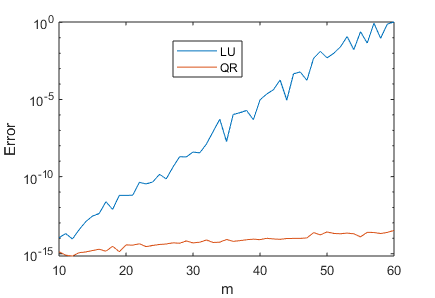
\includegraphics{ejer6bc.png}
	\caption{Comparación de los errores usando las descomposiciones QR y LU.}
\end{figure}

El error usando la descomposición $LU$ crece muchísimo más rápido que el de $QR$. Sabemos que la matriz $U$ tiene entradas que crecen del orden de $2^{m}$, por lo que su factor de crecimiento $\rho$ y el error en la resolución de ecuaciones también crecen exponencialmente.

Por otro lado, el error de resolver sistemas emplenado la factorización $QR$ depende del número de condición, precisamente, el error es del orden $O(\kappa(A)\epsilon_{m\'aq})$ (un resultado visto en clase). Hay que obtener $\kappa(A)=\Vert A\Vert_\infty\Vert A^{-1}\Vert_\infty$. Un cálculo nos dice que
\[
	A^{-1}=
	\begin{bmatrix}
		\frac{1}{2} & -\frac{1}{4} & -\frac{1}{8} & \cdots & -\frac{1}{2^{m-1}} & -\frac{1}{2^{m-1}}     \\[2pt]
		0           & \frac{1}{2}  & -\frac{1}{4} & \cdots & -\frac{1}{2^{m-2}} & -\frac{1}{2^{m-2}} \\[2pt]
		0           & 0            & \frac{1}{2}  & \cdots & -\frac{1}{2^{m-3}} & -\frac{1}{2^{m-3}} \\[2pt]
		\vdots      & \vdots       & \vdots       & \ddots & \vdots             & \vdots             \\[2pt]
		0           & 0            & 0            & \cdots & \frac{1}{2}        & -\frac{1}{2}       \\[2pt]
		\frac{1}{2} & \frac{1}{4}  & \frac{1}{8}  & \cdots & \frac{1}{2^{m-1}}  & \frac{1}{2^{m-1}}
	\end{bmatrix}
\]
(el patrón se sigue en las primeras $m-1$ columnas, y se rompe en la última). Puede verificar que esta es la inversa realizando el producto $AA^{-1}$. Como la norma-$\infty$ de matrices es el máximo de las normas-$1$ de cada fila, y como la norma-1 de cada fila es precisamente 1, entonces vemos que $\Vert A^{-1}\Vert_\infty=1$. Por otro lado, se calcula fácilmente que $\Vert A\Vert_\infty=m$. Por tanto $\kappa(A)=m$, es decir, el número de condición condición crece linealmente. Esto justifica que el error empleando la descomposición $QR$ sea mucho menor que aquel de emplear la descomposición $LU$.